%%%%%%%%%%%%%%%%%%%%%%%%%%%%%%%%%%%%%%%%%%%%%%%%%%%%%%%%%%%%%%%%%%%%%%
%%                     And
%%%%%%%%%%%%%%%%%%%%%%%%%%%%%%%%%%%%%%%%%%%%%%%%%%%%%%%%%%%%%%%%%%%%%%
%\color{blue}
\subsubsection{Glyph: \glyph{And}}\label{sec:and}

The glyph \glyph{and} is used to denote that all the \glyph{entity nodes} linked as input are necessary to produce the output influence.

\begin{glyphDescription}

 \glyphSboTerm SBO:0000173 ! and.

 \glyphContainer \glyph{And} is represented by a circle, with two connectors located at the opposite side for inputs and output.

  \glyphLabel \glyph{And} is identified by the label ``AND'' placed in an unbordered box attached to the center of the container. 

  \glyphAux \glyph{And} does not carry any auxiliary items.

\end{glyphDescription}


\begin{figure}[H]
  \centering
  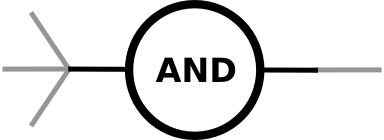
\includegraphics[scale = 0.5]{images/and}
  \caption{The \ER glyph for \glyph{and}. Three inputs are represented, but two or more than three would be allowed.}
  \label{fig:and}
\end{figure}

%\normalcolor
